\chapter{总结与展望}
\section{论文总结}
近几年的量子计算机的发展方向是规模化拓展以及尝试容错计算。
这些软硬件的发展,对量子系统的可靠性提出了更高的要求。
而量子模型检测是验证量子系统可靠性的一种自动化方法。其面临的主要困难是随着量子系统中量子比特增加,资源需求指数增长。

% 在本文工作中,通过应用新的数据结构,TDD,降低了量子模型检测的资源消耗。为未来量子计算机的验证提供了更好的工具支撑。
% 本文工作对量子系统的验证工作做出了一部分贡献,在量子硬件与软件快速发展的大背景下,满足了对有效验证技术不断增长的需求。
% 迁移系统是模型检测中的一种常用方法。而一步迁移算法对于模型检验,无论是经典还是量子迁移系统,都至关重要。
% 在本文工作中,将量子系统建模为量子迁移系统,探究了其可达空间的计算。
% 之后设计了基于TDD的子空间算法
% 同时本次工作专注于量子迁移系统中一步迁移算法过程中的资源爆炸问题。
本次研究的目的是设计更高效的量子模型检测工具。
而在TDD的数据结构基础上,本次研究设计了有效识别给定子空间基的算法,并针对子空间及量子线路,提出了多种优化策略。
基于此,本次研究设计了基于python的软件工具。
该软件工具的模块化设计保证了工具的拓展性,同时其中算法模块包含的优化方案也提高了计算效率。
% 这些工作为量子模型检测中的可达空间计算奠定了基础。

最后以量子迁移系统中一步迁移算法为例,本次研究设计了数值实验。实验结果验证了本次研究中软件工具的可行性,以及优化方案的效率提升。
特别地,数值实验还验证了采用基于contraction的线路分割算法能大幅提升量子迁移系统中一步迁移算法的效率。
% 通过将这些方法融合,并基于TDD的表示,最终设计了实验从而讨论关于一步迁移过程的资源需求。
% 这些工作进一步保证了TDD表示在量子模型检测中的实用性。
% 同时经过实验评估证明,


\section{工作展望}

% 在未来,伴随量子计算的不断发展,关于验证量子系统,比如量子线路和量子系统的工作会越来越重要。
% 本文研究过程中使用TDD表示对量子模型检测进行一定程度的探索,但仍然有以下工作需要完善。
% \begin{enumerate}
%     \item 在本次工作中,主要涉及量子迁移系统中的可达空间。在后续工作中,计划利用本文的方法关注那些只可以通过时态逻辑表述的属性。
%     \item 在本次工作中,主要涉及了可以用量子线路描述的描述系统。在后续工作中,还需要更深入探讨更为复杂系统的量子系统,特别是那些无法仅以量子线路形式表达的系统。
%     \item 在本次工作中,展示了对TDD优化而提高效率的实例。后续工作中应进一步提高TDD的表示能力,如利用一些特殊的张量等价关系。同时本次研究中主要使用的是基于python开发的TDD。在后续工作中,应当使用更高效率的程序语言,如C语言重新设计TDD,从而提高TDD的运算能力。
% \end{enumerate}
在未来,伴随量子计算的不断发展,验证量子系统(如量子线路和量子系统)的工作将变得越来越重要。本文在研究过程中使用了TDD对量子模型检测进行了初步探索,但仍有以下几个方面需要进一步完善。

在未来的工作中,可以利用本文的方法关注那些只能通过时态逻辑表述的属性。在本次工作中,主要涉及的是量子迁移系统中的可达空间。然而,许多量子系统属性只能通过时态逻辑来描述,这些属性对于确保量子系统的正确性和可靠性至关重要。未来的研究将致力于开发和应用新的方法,以便更有效地验证这些属性,确保量子系统在复杂应用中的安全性和有效性。

此外,未来的工作还需要深入探讨更为复杂的量子系统,特别是那些无法仅以量子线路形式表达的系统。本次研究主要集中在可用量子线路描述的系统上,而许多实际的量子系统要复杂得多,可能包含多种量子态和操作。进一步的研究将专注于这些复杂系统,开发适用于各种量子系统的验证方法,确保在更广泛的应用中验证量子系统中的命题。

最后,未来的工作应进一步提高TDD的表示能力,例如利用一些特殊的张量等价关系。本次研究展示了通过TDD优化提高效率的实例,但这只是一个起点。未来的研究将探讨如何利用更多的数学和计算工具来增强TDD的功能和效率。此外,本次研究主要使用的是基于Python开发的TDD。为了提高TDD的运算能力,后续工作中应当考虑使用更高效的编程语言,如C语言,重新设计和实现TDD。这将显著提升TDD的性能,使其能够处理更大规模和更复杂的量子系统。

综上所述,伴随量子计算的不断进步,量子系统的验证工作将变得越来越重要。本文在使用TDD进行量子模型检测方面进行了初步探索,但仍有许多需要完善和改进之处。未来的工作将重点关注时态逻辑属性的验证,深入探讨更复杂的量子系统,并提升TDD的表示能力和运算效率。通过这些努力,期望能为量子计算领域的发展提供更加坚实的基础,推动量子技术在各个领域的广泛应用。
% 在技术实现上,构建了两个版本的量子线路转化为TDD的工具,分别基于C语言和Python语言。这些工具的开发对于实现的研究方法至关重要,提高了实验的灵活性和效率。
% 其中的C语言的TDD支持任意维度张量,例如对双比特CNOT门,既可以按图\ref{fig:cnot-4}中的张量维度为4,
% 即按照索引为$q_1,q_0$进行表示。也可以按图\ref{fig:cnot-2}中的张量维度为4,
% 即按照索引为$q_3,q_2,q_1,q_0$进行表示。这样的设计大大提高了TDD的表示能力,为更复杂系统的验证提供了基础。
% \begin{figure}[!htbp]
%     \centering
%     \begin{subfigure}[b]{.4\textwidth}
%         \centering
%         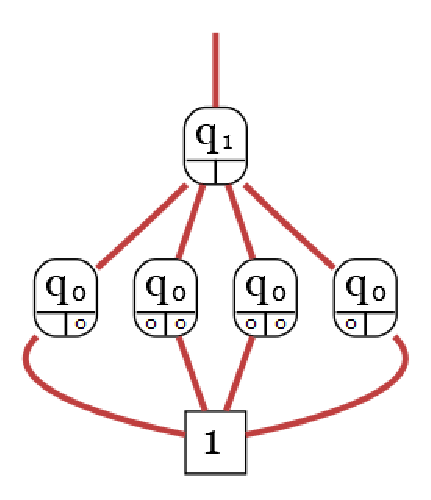
\includegraphics[height = 6cm]{Img/cnot.eps}
%         \caption{张量维度为4的CNOT门的TDD表示}
%         \label{fig:cnot-4}
%     \end{subfigure}
%     \begin{subfigure}[b]{.4\textwidth}
%         \centering
%         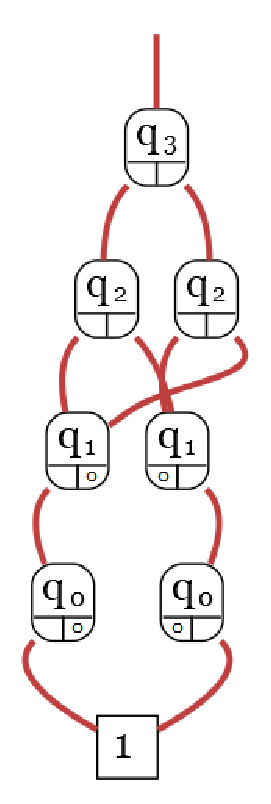
\includegraphics[height=6cm]{Img/cx.eps}
%         \caption{张量维度为2的CNOT门的TDD表示}
%         \label{fig:cnot-2}
%     \end{subfigure}
%     \caption{C语言版的TDD支持任意维度的例子}
%     \label{fig-cnot}
% \end{figure}
% \subsection*{limdd的改进}
% 由于量子状态都在同一希尔伯特空间中。因此作用某些算子后,不同的量子状态可能等价。
% 当存储算子的资源少于存储状态的资源时,就有可能存储算子表示不同的状态\citep{vinkhuijzen2023limdd}。图\ref{fig:qmdd-example}表示了一个QMDD的例子,应用等价性,可以化简为图\ref{fig:limdd-example}。
% TDD也可以应用类似技术,进行进一步化简,从而降低资源要求。
% \begin{figure}[!htbp]
%     \centering
%     \begin{subfigure}[b]{.4\textwidth}
%         \centering
%         \includegraphics[height=8cm]{Img/limdd.pdf}
%         \caption{一个QMDD示例}
%         \label{fig:qmdd-example}
%     \end{subfigure}
%     \begin{subfigure}[b]{.4\textwidth}
%         \centering
%         \includegraphics[height=8cm]{Img/limdd_reduce.pdf}
%         \caption{应用等价性化简图\ref{fig:qmdd-example}}
%         \label{fig:limdd-example}
%     \end{subfigure}
% \end{figure}
% \textcolor{red}{limdd的原理}